\chapter{Assessment of Entry Guidance for SRP-Based EDL}\label{Ch:FuelOptimalAssessment}
In order to characterize the behavior and performance of the propellant optimal entry guidance algorithm presented in Chapter~\ref{Ch:FuelOptimalPaper}, simulations are conducted under various circumstances. In all examples, the vehicle under consideration has a nominal $L/D=0.24$, and a ballistic coefficient of $310\, \mathrm{kg/m^2}$, approximately double that of Mars 2020. The vehicle's propulsion model includes an initial $ T/W $ of 4 with a constant $ I_{sp} = 290$ s, and $T_{\min}=0.5T_{\max}$. These parameters are summarized in Table~\ref{table_model_params}.
\begin{table}[h!]
	\centering
	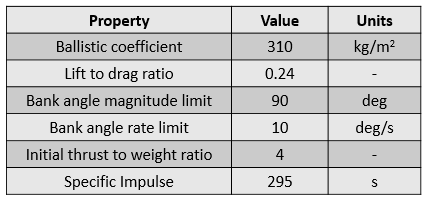
\includegraphics[width=0.6\textwidth]{../AAS20/ParamTable} 
	\caption{Model parameters used in all simulation results presented.}
	\label{table_model_params}
\end{table}
The site targeted at the termination of the descent phase is 700 km downrange with $z_{\mathrm{target}}=\dot{z}_{\mathrm{target}}=0$. 
%The entry flight path angle in all examples is $ -15.75^\circ $. The vehicle's bank angle rate is limited to $10 ^{\circ}/s$. 
Performance is evaluated using the propellant mass fraction (PMF), the portion of the vehicle that is propellant, as the primary metric. The bounds used in the constraints Eq.~\ref{eq_constraints} are $z_{\min} = 3$ km, $[d_{\min},\,d_{\max}] = [0, 25]\,$ km, $v_{\max} = 700 $ m/s. The entry phase terminates at the ignition velocity last predicted by the entry guidance algorithm.

\subsection{Sensitivity Analysis}
The performance of the algorithm is first investigated in a series of one-dimensional sensitivities to parametric uncertainties, including lift and drag coefficients, and two forms of density uncertainty. For this section, the atmospheric density is modeled as 
\begin{align}
\rho = \rho_0\mathrm{e}^{-\frac{R-R_P}{h_s}}
\end{align}
where $\rho_0 = 0.0158 \,\mathrm{kg/m}^3$ is the density at the surface and $h_s = 9354.5$ m is the scale height. Uncertainty is modeled in each of these quantities. Variations in $\rho_0$ correspond to constant percentage shift at all altitudes, while variations in the scale height alter the density's gradient with respect to altitude, $\dfrac{\partial\rho}{\partial h} = -\dfrac{\rho}{h_s}$. The guidance algorithm is called at four fixed velocities, $5500, 4000, 2000,$ and $1000$ m/s.
%Entry state dispersions are also examined. 

Due to its reliance on predictions, the algorithm is susceptible to model uncertainty. Reference~\cite{predictor_corrector_analysis} examined the performance of predictive algorithms in the presence of such uncertainties and found, like Ref.~\cite{lu2014entry}, that model adaptation during flight is essential to good performance in the presence of such parametric uncertainty. In the simulations presented, trajectory predictions are made aerodynamic accelerations scaled ratios of current sensed accelerations to modeled accelerations, $L/L_{model}$ and $ D/D_{model} $. Because the first three perturbations result in constant ratios of $L/L_{model}$ and $ D/D_{model} $, the predictions will match the simulated environment, and the predicted propellant consumption and ignition state should not vary significantly with each call to the entry guidance algorithm. In contrast, the scale height uncertainty will result in aerodynamic ratios that vary with altitude, causing error in the predictions due to their inability to account for unknown future variations. Thus it is expected to see greater variation in the predicted propellant required as well as the predicted ignition state. This behavior is exhibited in Fig.~\ref{fig_parametric_updates}.
\begin{figure}[h!]
	\centering
	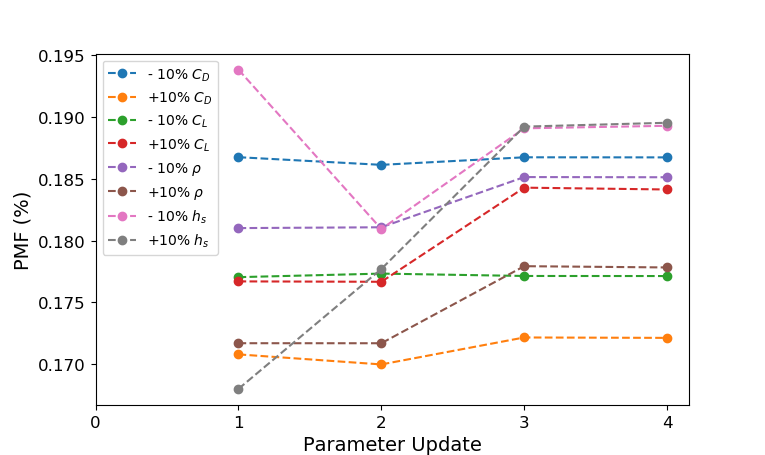
\includegraphics[width=0.7\textwidth]{../AAS20/ParameterUpdates} 
	\caption{The predicted PMF and associated ignition state may change each time the guidance algorithm is called. The solutions are less volatile when the discrepancy between the model predictions and the simulated environment is small. Larger variations in the solution due to variations in $h_s$ are expected since they result in unknown future density variations.}
	\label{fig_parametric_updates}
\end{figure}
\begin{table}[h!]
	\centering
	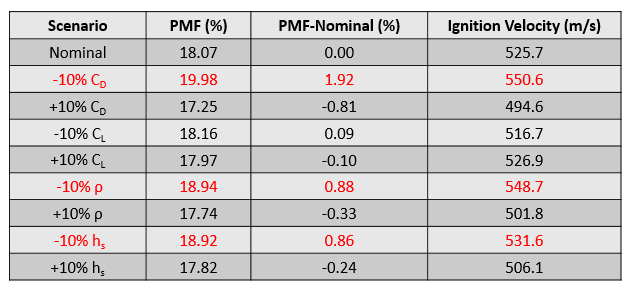
\includegraphics[width=0.75\textwidth]{../AAS20/ParametricSensitivityTable} 
	\caption{A summary of PMFs for a series of $\pm10\%$ uncertainties compared to a nominal scenario with no uncertainty. Scenarios with significant increases in PMF relative to the nominal scenario have been highlighted.}
	\label{table_parametric}
\end{table}
\begin{table}[h!]
	\centering
	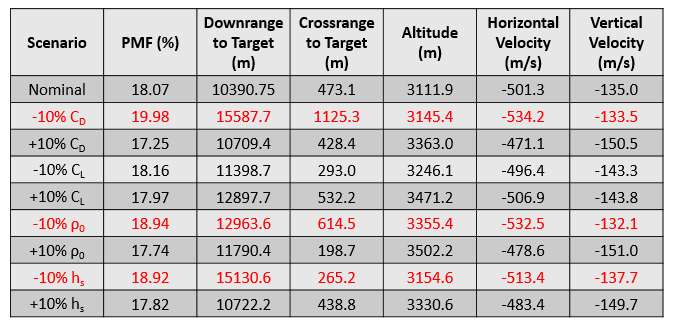
\includegraphics[width=0.8\textwidth]{../AAS20/ParametricSensitivityIgnitionTable} 
	\caption{A summary of the propellant-optimal ignition states for a series of $\pm10\%$ uncertainties. Optimal trajectories generally feature low crossrange, and altitudes close to the minimum altitude constraint.}
	\label{table_parametric_ignition}
\end{table}
\begin{figure}[h!]
	\centering
	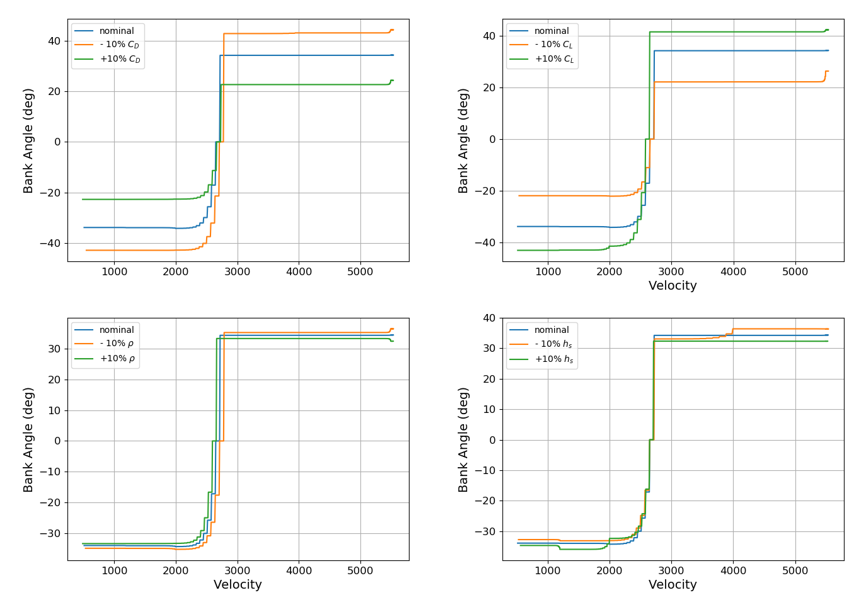
\includegraphics[width=0.9\textwidth]{../AAS20/SensitivityBankProfiles} 
	\caption{The bank angle profiles for a series of 1-D parametric sensitivities. Despite their similar effect on drag, the controller deals with $\pm C_D$ quite differently than $\pm \rho$.}
	\label{fig_parametric_bank}
\end{figure}

Figure~\ref{fig_parametric_bank} shows the resulting bank angle profiles. Due to their similar effect on the vehicle L/D ratio, the perturbations pairs  ($ +C_D $, $ -C_L $) and ($ -C_D $, $ +C_L $) result in essentially the same update to the bank angle magnitude. The lift dispersed cases essentially fly identical altitude-velocity profiles but have slightly different reversal velocities due to the impact of lift on lateral motion. 

Table~\ref{table_parametric} summarizes the PMF for each scenario and compares them to the nominal scenario, while Table~\ref{table_parametric_ignition} gives the corresponding propellant-optimal ignition states. Several trends are noticeable. The three scenarios with the highest PMF all involve lower than nominal drag acting on the vehicle, leading to higher ignition velocities and less favorable ignition states. Although the $-10\%\, \rho_0$ case features the same decrease in drag as $-10\%\,C_D$, it also preserves the $L/D$ ratio. Unlike the drag coefficient variations, the lift coefficient variations produced very little change in PMF.
There is a noticeable asymmetry present in each of the dispersions that affects drag: the minus variation, or ``low drag" scenario, requires a greater increase in PMF than is saved in the positive variation. Note that a constant $-10\%$ variation in drag (from any source) over the entire trajectory is a substantial perturbation that is challenging to overcome in the already thin atmosphere. Despite this, the additional PMF required relative to the nominal scenario is modest.

All of the trajectories feature lofting near the end of the entry phase (not shown), and the terminal altitude is almost always very close to the minimum altitude constraint. Since altitude decreases monotonically with velocity after lofting, this allows the vehicle to decelerate for as long as possible, reducing the velocity that must be nulled by SRP. Scenarios in which the optimal ignition occurs higher indicate some other constraint is active, such as overshooting the optimal downrange distance at which to ignite. Although there is no separate guidance logic for heading alignment, it is clear from the small crossrange values in Table~\ref{table_parametric_ignition} that by targeting the optimal point in $\mathcal{F}_M$, the vehicle heading is aligned prior to ignition. 

% For a fixed ground target, a wide range of entry flight path angles (EFPAs) and entry heading errors can be accommodated by the entry guidance algorithm. Figure~\ref{fig_sweep} is an example that demonstrates the propellant cost is approximately invariant with respect to entry azimuth errors and varies weakly with EFPA, about 200 kg of propellant over $1.4^\circ$ of variation in EFPA. The range of acceptable EFPAs is often set by considerations such as g-load limits, or aerothermal constraints, and these results indicate such constraints can be imposed at little-to-no cost to propellant. 
%
%It is expected that a guidance algorithm that provides range control during entry to the same downrange distance over such a range of EFPAs will fly very different entry trajectories with a much greater variance in the propellant cost to decelerate the vehicle while landing at the target. This is significant because vehicle designers will allocate propellant based on $3\sigma$ or high percentile estimates, and reducing both the mean and variance means potential for landing greater payload masses. A numerical assessment to quantify these effects...
%
%\begin{figure}[h!]
%	\centering
%	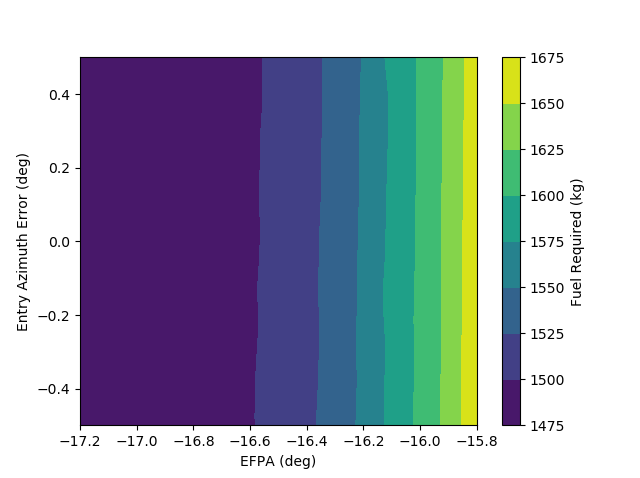
\includegraphics[width=1\textwidth]{optimal_fuel} 
%	\caption{Propellant required for different entry flight path angles and heading angles.}
%	\label{fig_sweep}
%\end{figure}

\subsection{Monte Carlo Simulation}
\begin{table}[h!]
	\centering
	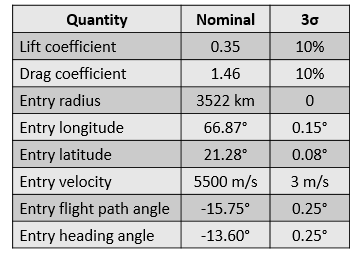
\includegraphics[width=0.4\textwidth]{../AAS20/DispersionTable} 
	\caption{The mean and $3\sigma$ values of the inputs used for the Monte Carlo simulation.}
	\label{table_input_dispersions}
\end{table}
\begin{figure}[h!]
	\centering
	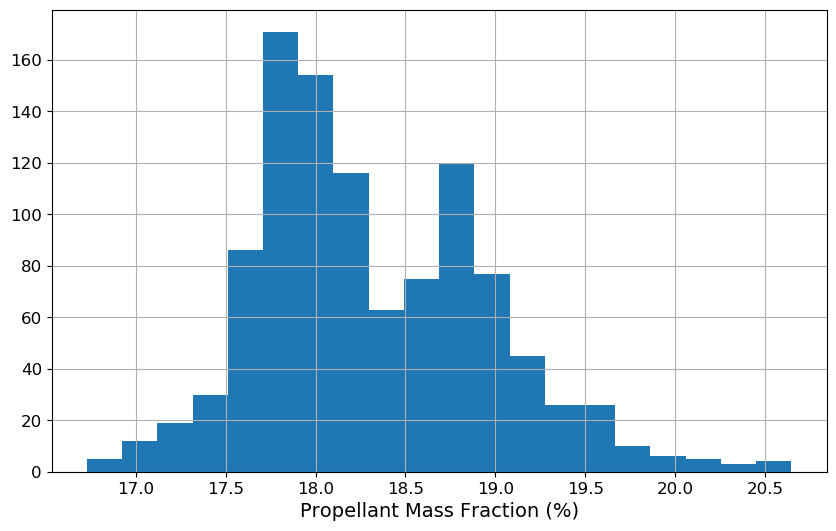
\includegraphics[width=0.6\textwidth]{../AAS20/ignition_pmf} 
	\caption{Propellant mass fraction for the Monte Carlo samples.}
	\label{fig_mc_pmf}
\end{figure}
\begin{figure}[h!]
	\centering
	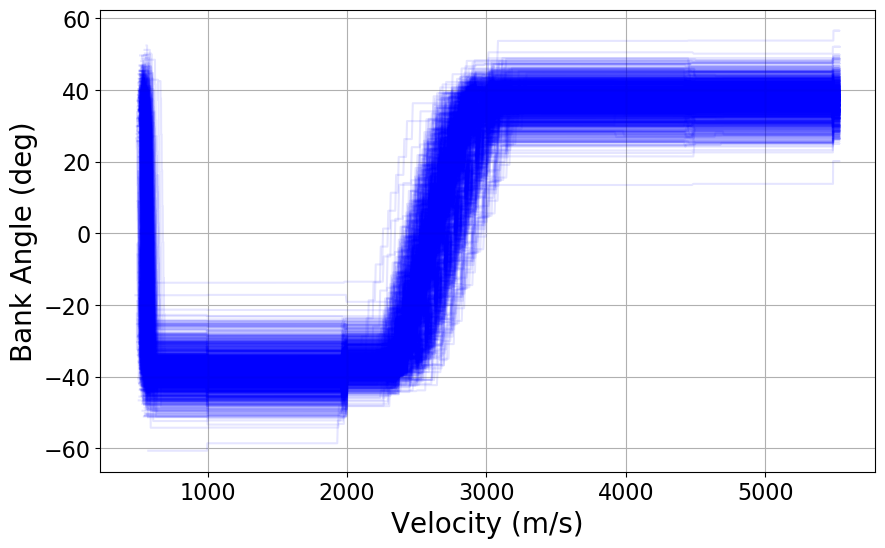
\includegraphics[width=0.6\textwidth]{../AAS20/bank_vel} 
	\caption{Bank angle profiles resulting from calls to the guidance algorithm at $ V=[5490, 4500, 3000, 2000, 1000] $ m/s.}
	\label{fig_mc_bank}
\end{figure}
\begin{figure}[h!]
	\centering
	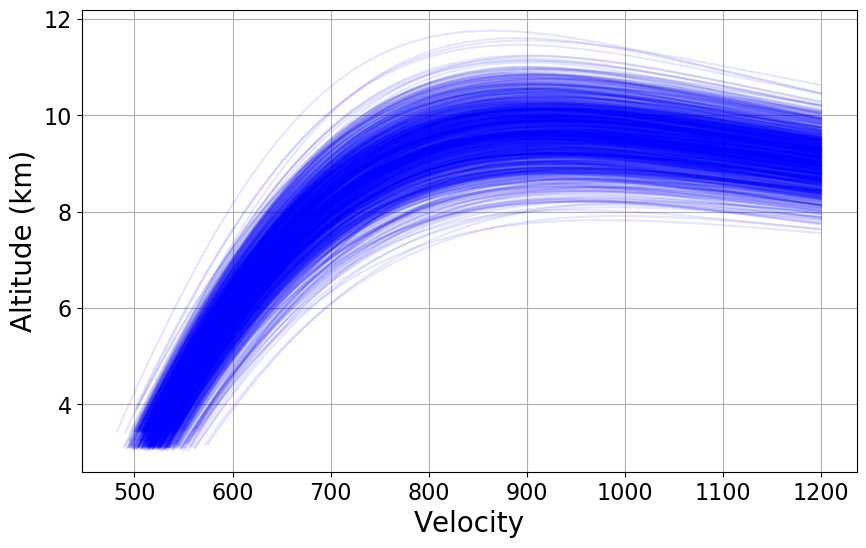
\includegraphics[width=0.6\textwidth]{../AAS20/alt_vel_zoomed} 
	\caption{All of the trajectories feature lofting as a means to further decelerate prior to ignition.}
	\label{fig_mc_alt_vel}
\end{figure}
\begin{figure}[h!]
	\centering
	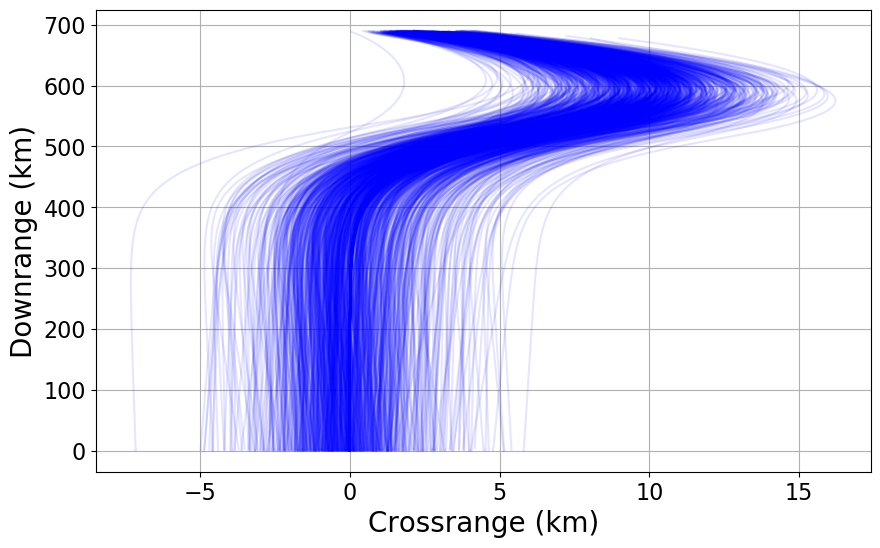
\includegraphics[width=0.6\textwidth]{../AAS20/dr_cr} 
	\caption{Downrange and crossrange flown from the entry state. Some trajectories fly significant crossranges due to the single planned bank reversal. Note that there are initial downrange errors in addition to than the initial crossrange errors, but due to the difference in scale they are not easily visible.}
	\label{fig_mc_entry_dr_cr}
\end{figure}
\begin{figure}[h!]
	\centering
	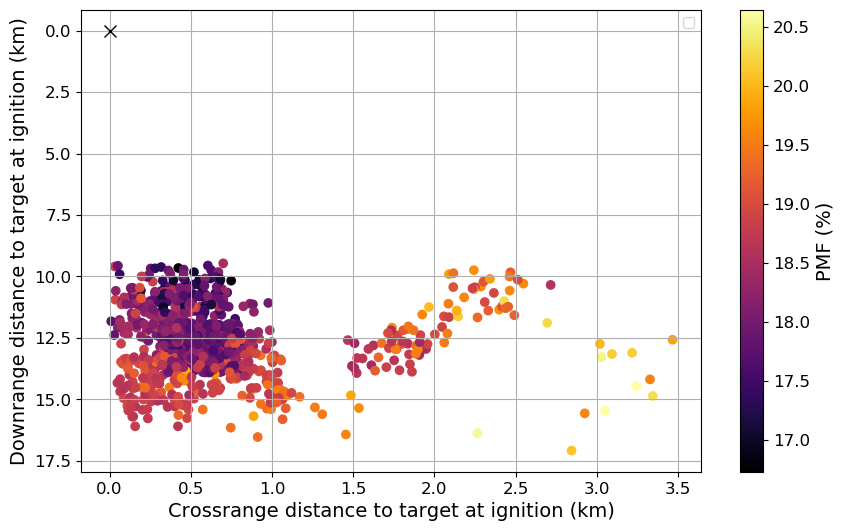
\includegraphics[width=0.7\textwidth]{../AAS20/ignition_dr_cr} 
	\caption{Downrange and crossrange to the target position. The crossrange is generally small, with 88\% under 1 km, indicating the vehicle heading is well-aligned at ignition.}
	\label{fig_mc_ignition_dr_cr}
\end{figure}
\begin{figure}[h!]
	\centering
	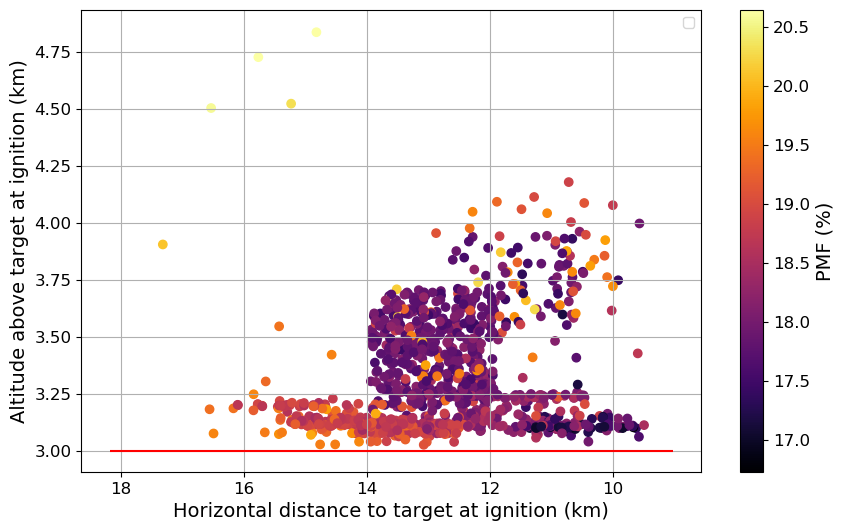
\includegraphics[width=0.7\textwidth]{../AAS20/ignition_alt_range} 
	\caption{The minimum altitude constraint, indicated in red, causes low energy scenarios to trigger at longer downrange distances and higher velocities, resulting in increased PMF.}
	\label{fig_mc_ignition_alt_vs_distance}
\end{figure}
\begin{figure}[h!]
	\centering
	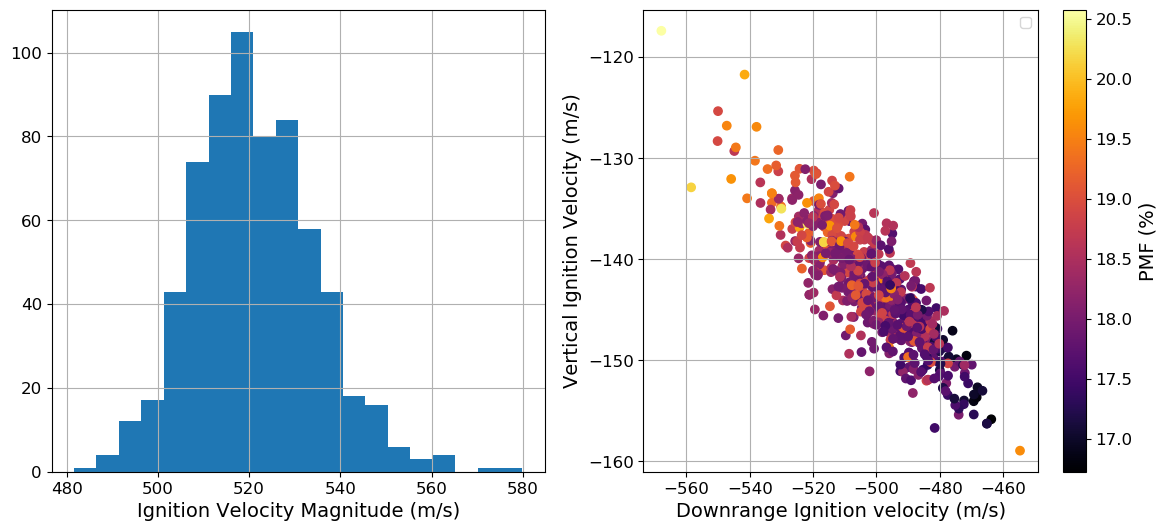
\includegraphics[width=0.9\textwidth]{../AAS20/ignition_vz_vx} 
	\caption{Ignition velocity magnitude (left) and components (right). Lower ignition velocities tend to occur at steeper flight path angles for the chosen parametrization. The correlation between velocity and PMF is evident, but the slowest ignition point (bottom right of the right plot) is nowhere near the lowest PMF value, demonstrating the importance of other state variables in determining the PMF required.}
	\label{fig_mc_ignition_vel}
\end{figure}
A Monte Carlo of 1000 samples is conducted with entry state delivery errors and aerodynamic dispersions, listed in Table~\ref{table_input_dispersions}, and a higher fidelity atmosphere model. The atmospheric density is modeled using MarsGRAM \cite{MarsGRAM2010User}, rather than the exponential model employed specifically for the sensitivity study. 
 
Figure~\ref{fig_mc_pmf} shows the distribution of PMFs and
Figs.~\ref{fig_mc_bank}-\ref{fig_mc_entry_dr_cr} display the entry trajectories. The median PMF is 18.2 \%, and the 99 percentile is 20.1\%. From Fig.~\ref{fig_mc_alt_vel} it is evident that all of the samples feature at least a mild lofting near the end of the entry phase. 
Figure~\ref{fig_mc_bank} depicts the bank angle profiles. The chosen parametrization of the bank profile, coupled with the nature of the disturbances modeled, means that unless significant perturbation of the vehicle heading occurs after the first reversal, there will be only one reversal in total. In instances where the prediction was inaccurate and the reversal was poorly timed as a result, a late second reversal is used to correct the vehicle heading. 

Figures~\ref{fig_mc_ignition_dr_cr}-\ref{fig_mc_ignition_vel} plot the ignition states at the ignition velocity determined by the last call to the entry guidance algorithm. For the vehicle under consideration, the optimal downrange to the target is generally between 10-15 km. Nearly all samples have a crossrange distance of less than 1 km at ignition, and the maximum crossrange samples trigger with around 3.5 km crossrange to the target. As seen in Fig.~\ref{fig_mc_ignition_vel}, ignition velocities occur over a range of nearly 100 m/s. PMF and velocity at ignition are naturally correlated, but the lowest velocity ignition (the point in the bottom right of the right plot) is near the upper end of the PMF range, which shows that other state variables may yet have a strong impact on the PMF required to land.

Figure~\ref{fig_mc_ignition_alt_vs_distance} shows that altitude at ignition is consistently low, within 1-2 km of the minimum altitude constraint. This is not surprising, as after the vehicle has passed the point of lofting, the lowest velocity along an entry trajectory will occur at the minimum altitude.
% Thus, low altitude ignitions are known to be optimal when the ignition flight path angles are shallow ($\le20^{\circ}$). 
%While this is the case for propellant-optimal powered descent solutions, it may not be true generally, i.e., for an alternative powered descent guidance. Nevertheless, 
The consistently low ignition altitudes suggest a guidance strategy that triggers ignition at a fixed altitude may perform nearly as well as searching for the optimal ignition state. Doing so would eliminate the need to find the optimum ignition point along a trajectory, removing the nested computation structure, and leaving only the optimization over the parameters of the bank angle profile. An additional benefit of such a strategy is a reduction of the propellant mapping interpolation to four dimensions, requiring far fewer solutions to represent the mapping with the same accuracy. Additionally, some of the suboptimality associated with an altitude trigger would be mitigated by the vehicle flying slightly differently knowing that the ignition altitude is different. 

Reference~\cite{PropellantOptimalAdaptiveTrigger} also noted that propellant-optimal ignitions generally occur near the last feasible entry state, but submits that propellant consumption alone is not a sufficient criterion for powered descent ignition because it does not account for operational margins. We suggest alternatively that by defining the minimum altitude constraint with operational margin in mind, the entry guidance algorithm may utilize an altitude trigger and focus exclusively on propellant consumption without issue. Another possible generalization is to trigger on a fixed glideslope angle, essentially allowing the final altitude to be lower if the vehicle is also nearer to the target.

\begin{figure}[h!]
	\centering
	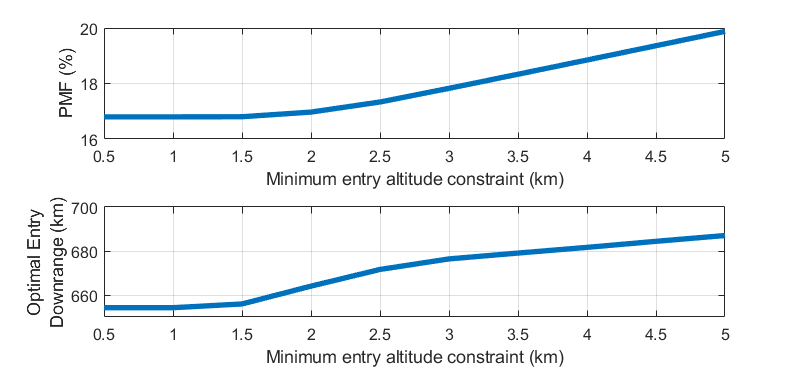
\includegraphics[width=0.9\textwidth]{../AAS20/min_alt_constraint} 
	\caption{The optimal placement of the target from the entry interface varies considerably with minimum entry altitude constraint has a strong impact on the geometry of the propellant optimal powered descent trajectories.}
	\label{fig_min_alt_constraint}
\end{figure} 
\begin{figure}[h!]
	\centering
	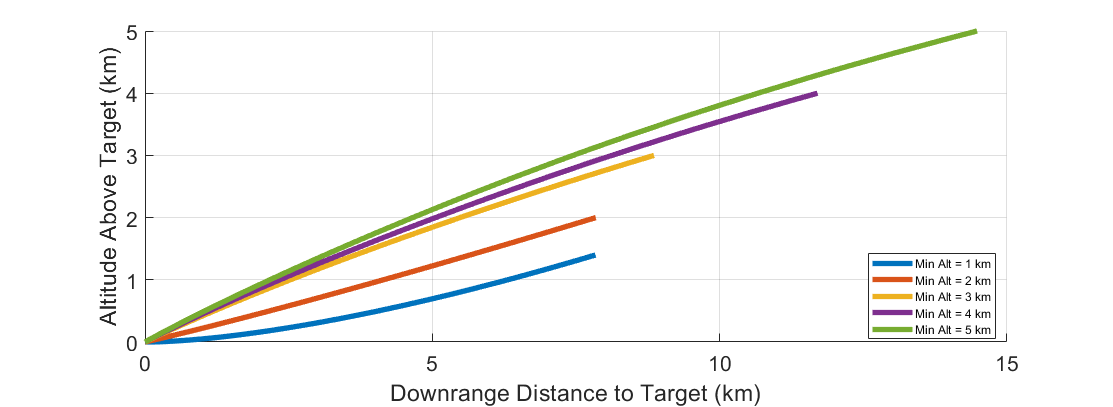
\includegraphics[width=0.9\textwidth]{../AAS20/SRP_vs_min_alt} 
	\caption{The minimum entry altitude constraint has a strong impact on the geometry of the propellant-optimal powered descent trajectories.}
	\label{fig_srp_traj}
\end{figure} 
 
 % %New stuff
The minimum altitude constraint also implications during mission design. Not only does it strongly affect the geometry of the powered descent phase, but it also affects the optimal entry trajectory length and the minimum propellant required.
 Figure~\ref{fig_min_alt_constraint} plots these quantities versus the value of the altitude constraint, while Fig.~\ref{fig_srp_traj} shows how the powered descent trajectories vary with the constraint. 
For the vehicle considered, and a constant bank angle magnitude during entry, the unconstrained optimal ignition altitude is about 1.5 km above the target. When the targeted downrange distance is free, the growth in PMF due to the constraint is modest, but the optimal entry downrange distance grows by nearly 40 km when imposing a 5 km constraint, and the propellant-optimal downrange distance from the target at ignition nearly doubles. 
 % %End New stuff
 
 
%\section{Discussion}
%An entry guidance algorithm for chuteless, retropropulsion-based entry, descent, and landing was proposed. In particular, we addressed the problem of steering an entry vehicle to a propellant-optimal ignition condition. Feasible solutions to the powered descent problem are used to define the entry guidance target set. By computing and storing a mapping from ignition states in the target set to propellant required, the entry guidance algorithm maintains a predicted ignition state that varies over time as various perturbations alter the reachable set of the vehicle. The guidance algorithm updates the bank profile in order to track the propellant-optimal reachable state.
%
%Although the role of entry guidance has always been to deliver the vehicle to favorable conditions for subsequent descent and landing phases, the use of the powered descent phase's guidance to define a target set, specifically for the purpose of reducing predicted powered descent propellant consumption, is novel. In parachute-based architectures, Mars entry guidance algorithms are generally judged on their ability to manage range errors while reaching the safe parachute deployment set. In contrast, in chuteless missions where pinpoint landing is achieved via powered descent, we posit that performance will instead be based on the required propellant to land the vehicle.
%
%In the presented approach, the transition from the entry phase to powered descent is determined onboard during the optimization of the bank angle profile, but numerical results suggest that a possible simplification of the trigger is possible with little to no increase in propellant. Using a fixed altitude trigger would remove the need to optimize the ignition point along individual trajectories, and would allow a further reduction in size of the propellant map due to the decrease in dimensionality of the possible ignition states. The approach was demonstrated using a simple parametrization. Future work will consider alternatives, such as a profile designed specifically for achieving low velocity, which will likely yield lower propellant consumption. 


%%% Local Variables: ***
%%% mode: latex ***
%%% TeX-master: "thesis.tex" ***
%%% End: ***
